\documentclass[a4paper]{article}

%--------------------------------------------------------------------------

\usepackage[a4paper, total={6in, 9in}]{geometry}
\usepackage{amsmath}
\usepackage{booktabs}
\usepackage{caption}
\usepackage{enumitem}
\usepackage{graphicx}
\usepackage{float}
\usepackage{inconsolata}
\usepackage{listings}
\usepackage{pstricks-add}
\usepackage{siunitx}
\usepackage[most]{tcolorbox}
\usepackage{tikz}
\usepackage{epstopdf} %converting to PDF
\usepackage[hidelinks]{hyperref}
\usepackage{makecell}
\usepackage{amssymb}
\usepackage{siunitx}
\usepackage{wrapfig}

\usetikzlibrary{shapes.geometric, arrows}

%------------------------------------------------------------
\setlength{\parindent}{0in}

%------------------------------------------------------------
\tikzstyle{block} = [draw, fill=blue!20, rectangle, 
minimum height=3em, minimum width=6em]
\tikzstyle{sum} = [draw, fill=blue!20, circle, node distance=1cm]
\tikzstyle{input} = [coordinate]
\tikzstyle{output} = [coordinate]
\tikzstyle{pinstyle} = [pin edge={to-,thin,black}]

%------------------------------------------------------------
\graphicspath{{./fig/}}

%------------------------------------------------------------

\begin{document}
\title{ENG417 Sustainability\\Should Australia have a population policy?}
\author{Shane Reynolds}
\maketitle
\tableofcontents

\newpage

%------------------------------------------------------------
\section{Introduction}

This paper investigates key elements of a population policy, discuses whether a population policy is suitable for Australia, and provides a population policy proposal based on the findings. Mathematical modelling is undertaken to provide insight on whether the proposed policy is possible, and to assess how it may perform. Finally, the implications of the population policy are explored surrounding the sustainability of Higher Education providers in Australia.

%------------------------------------------------------------
\section{Australian Population \& the Ideal Growth Rate}

Population policy refers to policy whereby the government seeks to directly, or indirectly, influence population determinants in order to deliberately alter the size, and growth rate, of the population \cite{NPC:1992}. Impressive though it may be for a government to alter the number of people it governs, population policy is not adopted for it's own sake. Government wields this tool to achieve goals which society at large, or government on its behalf, believe desirable and attainable \cite{IRS:1997}. One such goal is the preservation of the environment and sustainable use of natural resources. This is especially true in Australia, where the environment is fragile and resources limited: the arable share of land is small, water supplies are subject to large fluctuations due to seasonal variations in rainfall, fertile top soils are thin and vulnerable to depletion, and there are many threatened species of local flora and fauna \cite{Smith:2003}. Recently, the Australian population surpassed 25 million \cite{ABS1:2018}, and is forecast to reach 46 million by 2075 \cite{ABS2:2018} - how do we know if this is too many people? In contrast to motives of environmental preservation, a sustainable approach to population also requires economic considerations be made. A well cited article by Banerjee suggests increased population sizes have a drag effect on productivity gains enjoyed from technological innovations borne by research and development \cite{Banerjee:2012}. At the same time Banerjee acknowledges that as productivity increases natural rates of procreation fall which places increased economic penalty on younger members of society in the face of an ageing population. To ensure that an economy is not limiting the economic well-being of it's citizens requires a better understanding of the complex dynamics behind population growth. This section begins by identifying and defining carrying capacity, which can be used to help estimate desired population levels. Additionally, population growth rates are examined to provide a clear picture of instruments available so government can alter population size to desired levels.

\subsection{Carrying Capacity}
Carrying capacity is used to describe the total number of people that a land area can support. Fearnside describes this more formally as, ``the maximum number of persons that can be supported in perpetuity on an area'' \cite{Fearnside:1986}. Whilst there are many different approaches to estimating carrying capacity, they largely centre around calculations of the number of individuals that an area's food and water supply can support. Cohen provides a simple definition using the following mathematical expression \cite{Cohen:1995}:
\begin{equation*}
carrying \ capacity = \min \bigg\{ \frac{water \ supply}{individual \ water \ requirement} \ , \  \frac{food \ supply}{individual \ food \ requirement} \bigg\}
\end{equation*}

In theory, this is an ideal metric to help government find a basis for population policies, however, practically the measure is problematic for a number of reasons. Firstly, the definition of area means that boundaries need to be drawn from which there is no external trade \cite{Lane:2017}. Globalised economies often engage in specialisation and trade to boost economic performance. The implications are that it is possible, albeit risky, for a nation with arid land (unsuited for food production) to rely on services as their main economic output which can be traded for food, or other natural resources. This is one a way for a population to indefinitely exceed the carrying capacity of a region, assuming trade does not cease, and their services continue to be valued. Secondly, Cohen suggests that carrying capacity is notoriously hard to accurately estimate in the long term because technological developments increase productivity in unforeseen ways \cite{Cohen:1995}.\\

Difficulties estimating the carrying capacity metric are often cited as reasons why the Australian government has been reluctant to officially estimate Australia's carrying capacity. There have been some historical attempts, however. Thomas Griffith Taylor, in the early 1900s, estimated the carrying capacity to be around 20 million. Notably, he made his estimations without envisaging the expansion of global trade and technological progress, and the estimate is considered to be low by modern methods. More recently, in 1991, the National Population Council report estimated around 50 million as the maximum carrying capacity \cite{SCLTS:1994}. This took into account technological productivity gains, and allowed for some trade. This figure was revised downward to 30-35 million taking safety margins into consideration \cite{Lane:2017}.\\

Carrying capacity is useful for providing an indication on how many people a land area can support, and to that end is an important consideration when determining population policies. Ideally, it should be used as a guide for policy makers when determining what population size a country should be targeting.

\subsection{Growth Rate}
Carrying capacity yields insight on sustainable population sizes, however, it provides no comment on what population growth should look like to achieve a desired population size. The population growth rate, $r$, is defined as the percentage change in the population over some given time interval. If $P_i$ is the initial population, $P_f$ is the final population after some time interval, $\delta t = t_f - t_i$, then the population growth rate can be expressed mathematically as follows:
\begin{equation}
	r = \frac{P_f - P_i}{P_f \cdot (t_f - t_i)}
\end{equation}

Although Australia has never announced an official growth rate, the Australian Population and Immigration Council argue that Australia had a historical target growth rate of 2 percent from the postwar years until the early 1970s. The unofficial decision to hold this target was more to do with bolstering national security and economic prosperity than attempting to establish a desired population level. Increased pressures on infrastructure seen in Australia's major cities make it is less clear what growth rate Australia should be trying to achieve today. Currently the growth rate is approximately 1.7\%, however, this is not distributed throughout Australia equally with major capital city growth rates much higher than growth rates in regional centres \cite{ABS3:2018}. In order to make a recommendation on desirable growth rates, we first need to understand the main factors which influence it - our discussion will be limited to the two principal drivers of population growth: the natural rate of growth; and the net rate of migration.

\subsubsection{Natural Growth Rate}
The natural rate of growth, $r_n$, refers to the birth rate, $r_b$, less the death rate, $r_d$, which is sometimes referred to as the mortality rate. Whilst there are many different ways to measure the birth rate, this paper will employ the crude method. The crude birth rate is expressed as the percentage change in the population due to births per unit of time - this sees the population increase. As of 2017, the crude birth rate in Australia is 1.28\% \cite{ABS3:2018}. Figure 1 shows a longitudinal view of the crude birth rate in Australia from 1980 to 2010, calculated with data from the Australian Beureau of Statistics \cite{ABS4:2018}. Notably, the birth rate can be seen to be slowly declining, which is attributed to our slightly lower than replacement fertility rate of 1.8, and our ageing population.\\

\begin{figure}[h]
	\begin{minipage}[t]{0.45\textwidth}
		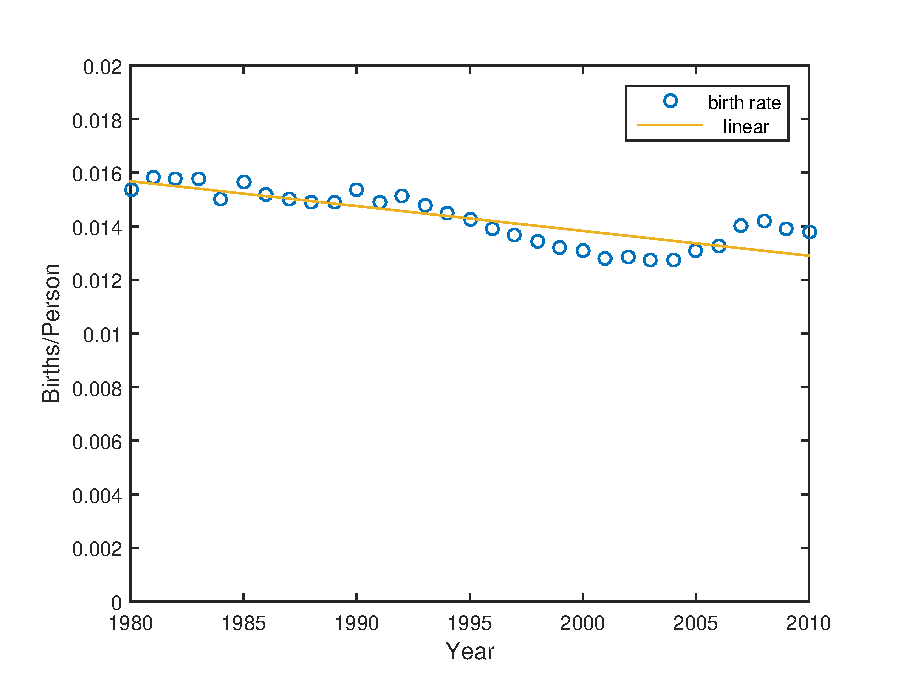
\includegraphics[scale=0.52]{birth_rate}
		\caption{Time series of the crude birth rate in Australia from 1980 to 2010}
	\end{minipage}
	\hspace{1cm}
	\begin{minipage}[t]{0.45\textwidth}
		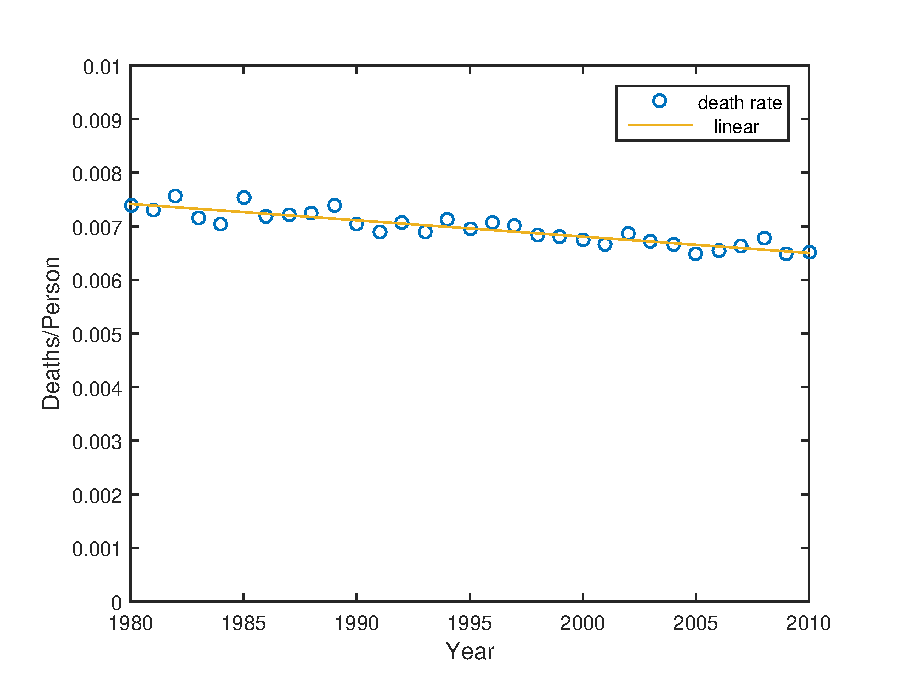
\includegraphics[scale=0.52]{death_rate}
		\caption{Time series of the crude death rate in Australia from 1980 to 2010}
	\end{minipage}
\end{figure}

The crude death rate is expressed as the percentage change in the population due to deaths, per unit of time - this sees the population decrease. As of 2017, the crude death rate in Australia is 0.67\% \cite{ABS3:2018}. Figure 2 shows a longitudinal view of the crude death rate in Australia from 1980 to 2010, calculated with data from the Australian Beaurea of Statistics \cite{ABS4:2018}. Like the birth rate, the death rate can be seen to be slowly declining, which is attributed to increases in life expectancy. Even though both the birth and death rates are decreasing the natural rate of growth is relatively static - this is because the negative drift in birth is cancelled out by the negative drift in the death rate. This means it's relatively safe assume the natural rate of growth is somewhat static. 

\subsubsection{Net Rate of Immigration}
The net rate of immigration refers to the net change in the population due to immigration and emigration, expressed as a percentage per unit of time. Specifically, it is the immigration rate, $r_i$ , less the emigration rate, $r_e$. The immigration rate represents inflows into Australia, and the emigration rate represents outflows of residents leaving Australia. We calculate the immigration and emigration rates using similar crude methods used to calculate the birth and death rates. It must be noted that, by ABS definition, immigration and emigration rates only consider permanent and long term movement in their figures. Figure 3 shows the longitudinal view of the crude immigration rate from 1980 to 2010 \cite{ABS5:2018}. A striking increase can be seen in the rate over the 10 year period - the rate has almost doubled.

\begin{figure}[h]
	\begin{minipage}[t]{0.45\textwidth}
		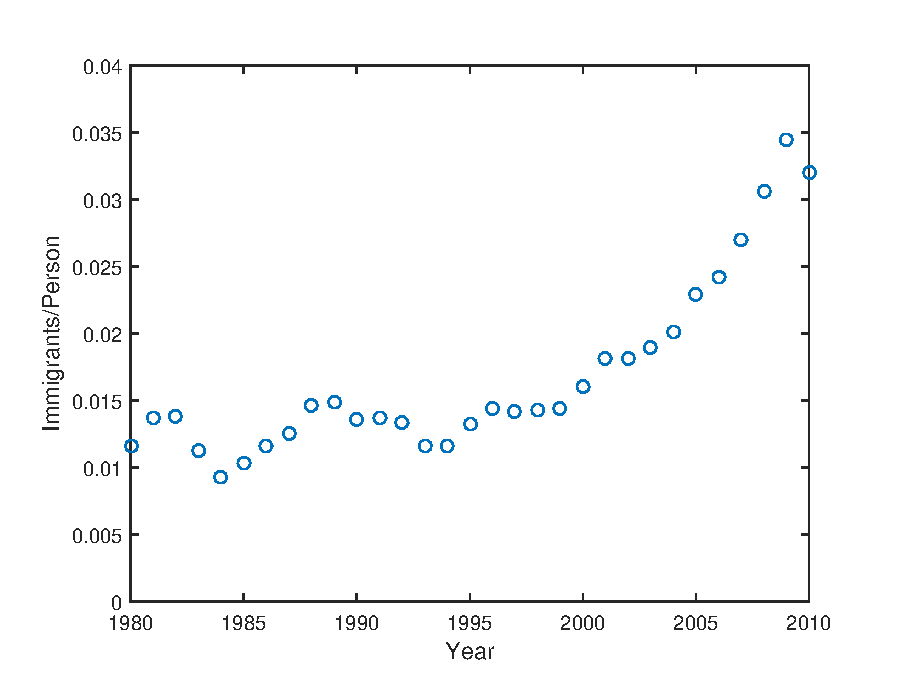
\includegraphics[scale=0.52]{immigration_rate}
		\caption{Time series of the crude immigration rate in Australia from 1980 to 2010}
	\end{minipage}
\hspace{1cm}
	\begin{minipage}[t]{0.45\textwidth}
		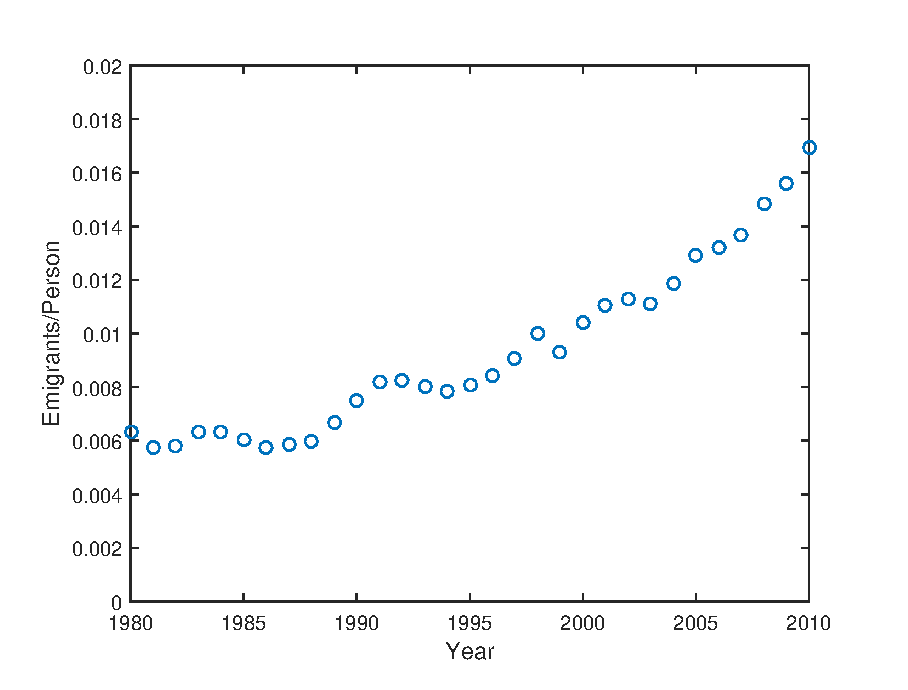
\includegraphics[scale=0.52]{emigration_rate}
		\caption{Time series of the crude emigration rate in Australia from 1980 to 2010}
	\end{minipage}
\end{figure}

Figure 4 shows a longitudinal view of the emigration rate from 1980 to 2010 \cite{ABS5:2018}. We note that the emigration rate has experienced similar increases when compared to the immigration rate. Increases seen in both immigration and emigration are are often attributed to the upwardly mobile populations of an increasingly globalised world (REFERENCE). 

\subsection{Recommendation for Australian Population Policy}
Based on the previous discussion, this paper proposes that Australia should be maintaining a growth rate at some point below $1.7\%$ to ensure our major capital cities can sustainably manage increasing demands on infrastructure, although this could be increased above $1.7\%$ provided the government imposes policies forcing regional settlement and restrictions on internal migration. Furthermore, the Australian government should make it a priority to determine a sustainable population level based on carrying capacity estimates, accounting for safety margins on food and water supplies. Finally, once a population level has been determined Australia should implement policy to drive the population to the desired level to maximise economic prosperity and citizen well-being. The implemented policy should not impinge on current freedoms enjoyed by Australian citizens and immigration should be the main policy lever employed to this end. It must be highlighted that population levels estimated from carrying capacity are not fixed and should be revised often as new technological innovation brings increased efficiencies.  


%------------------------------------------------------------

\section{Modelling the Population Policy}
Section 2.3 proposed that the Australian government could increase standard of living by implementing a population policy aimed at achieving desired population size, based on carrying capacity estimates, using a growth rate less than 1.7\%. The control of the population size and growth rate would be implemented using immigration rates. This section of the report uses mathematical modelling to determine if this policy is reasonable, or even possible. It is broken up into four subsections: Assumptions; Population Model; Population Control Policy; and Analysis of Results. 

\subsection{Assumptions} 
The biggest assumption made during this modelling is that the system population dynamics are linear and time invariant. Whilst the modelling used here does not violate the linearity assumption, it is questionable to assume that the model is time invariant particularly over the long term. Sections 2.2.1 and 2.2.2 showed that the birth, death, and emigration rates all vary with time. The drift seen in the birth and death rates are somewhat eliminated when calculating the natural growth rate, however, the immigration rate is used as a control mechanism in our modelling below meaning emigration rate time variance is present in the system. What makes matters worse is that this rate has seen dramatic increase over the last 10 years. The main implications for this assumption is that the modelling is only valid for the short term, and reliability of the results decreases the in the longer term.  

\subsection{Population Model}
One way to think about a country's population system is in terms of economic stock and flow, whereby the stock is the pool of people residing in a country at a given time, and the flows are the changes to the population due to the birth rate, mortality rate, emigration rate, and immigration rate. Using an engineering analogy to the classical tank flow problem allows us to represent this pictorially, as shown in Figure 5. The diagram shows that the population level of a country can be thought of as the level of water in a tank - the level changes due to the various inflows and outflows depicted. One interesting addition to the diagram is the implementation of flow control valve on the immigration inflow. As discussed in Section 2.3 this represents the governments only method of attempting to control population which does not impinge on the current freedoms enjoyed by residents.\\

\begin{figure}[h]
	\centering
	\includegraphics[scale=0.5]{tank_flow}
	\caption{Classical engineering tank flow control problem used as an analogy to describe the population in Australia. The population is represented as the level of fluid in the tank. Births and immigration represent inflows to the population, and deaths and emigration represent outflows from the population.}
\end{figure}

To aid analysis of a country's population dynamics, we can develop a mathematical expression for the system depicted in Figure 5. Suppose that the Australian population at some time $t$ is represented by $P(t)$. Additionally, we let $r_n$ represent the natural growth rate, $r_e$ represent the emigration rate, and $X(t)$ be the additional number of people let into the country, annually, from immigration. Note that the natural rate of growth, $r_n$, is calculated as the birth rate, $r_b$, less the death rate, $r_d$. Mathematically, this is expressed as:
\begin{equation}
r_n = r_b - r_d
\end{equation}

Assuming some incremental change in time, $\delta t$, the population at time $t + \delta t$ can be described by adapting the Malthusian equation:
\begin{equation}
P(t + \delta t) = P(t) + \delta t \cdot r_n \cdot P(t) - \delta t \cdot r_e \cdot P(t) + \delta t \cdot X(t)
\end{equation}

Rearranging equation (3) and considering the case when $\delta t \to 0$, we get the following differential equation:
\begin{equation}
\frac{dP(t)}{dt} = r_n \cdot P(t) - r_e \cdot P(t) + X(t)
\end{equation}

Equation (4) is a well known first order form, which is typically expressed as:
\begin{equation}
\frac{dP(t)}{dt} - (r_n - r_e) \cdot P(t) = X(t)
\end{equation}

Given the system input, $X(t)$, we expect a homogeneous and particular solution to emerge when we solve the system. The homogeneous solution is the response of the system from it's initial conditions, which is the initial population at time $t = 0$. The particular solution is the response of the system for the given input, $X(t)$. Given that the immigration policy, $X(t)$, is not clearly defined, it is more insightful to continue our analysis in the complex $s$-domain. Taking the Laplacian transform of equation (X), we can see the following:
\begin{align}
\mathcal{L} \bigg\{ \frac{dP(t)}{dt} \bigg\} - \mathcal{L} \{ (r_n - r_e) \cdot P(t) \} &= \mathcal{L} \{ X(t) \}\\
P(s) \cdot s - P(t)|_{t=0} - (r_n - r_e) \cdot P(s) &= X(s)
\end{align}

Rearranging equation (7), we get the following expression for the population system:
\begin{equation}
P(s) = \frac{P(t)|_{t=0}}{s - (r_n - r_e)} + \frac{1}{s - (r_n - r_e)} \cdot X(s)
\end{equation}

Taking the inverse Laplace transform results in an expression in the temporal domain:
\begin{equation}
P(t) = P(t)|_{t=0} \cdot e^{(r_n - r_e) \cdot t} + \mathcal{L}^{-1} \bigg\{ \frac{1}{s - (r_n - r_e)} \cdot X(s) \bigg\} 
\end{equation}

Equation (9) allows us to gain some insight on how the population system might respond if the government turned off immigration. We are able to observe this response if the government declared that there would be no further immigration into Australia. Mathematically would be equivalent to setting $X(t)$ to zero immigrants per year. Under this scenario, equation (9) would become:
\begin{equation}
P(t) = P(t)|_{t=0} \cdot e^{(r_n - r_e) \cdot t}
\end{equation}

We note from our earlier assumptions that $r_n - r_e < 0$. Hence, if there were no immigration, the initial population would fall asymptotically to zero, certerus paribus. This can be seen in Figure 6. Of course, the population decline shown in Figure 6 is unlikely to every occur since it is based on the unrealistic long term assumption of time invariance which sees birth, death, and emigration rates remain static. What this does imply, however, is that Australia's population could be controlled, using immigration as a control variable, over the short term. Essentially, if some desirable sustainable population size could be determined using existing estimates of carrying capacity, then this could employed as the desired set point for the population. The control policy would change the number of immigrants allowed in per year, $X(t)$, in order to meet the desired population set point.

\begin{figure}[h]
	\centering
	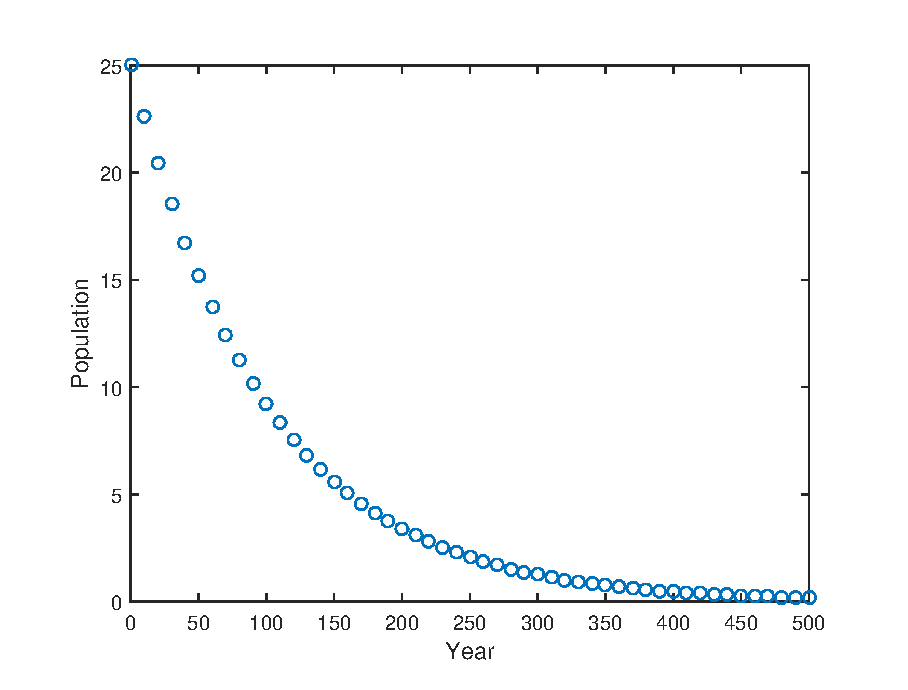
\includegraphics[scale=0.5]{population_decline}
	\caption{Assuming that the system is time invariant and $r_n < r_e$, then if the immigration rate is set to zero the population size will tend to zero, asymptotically.}
\end{figure}

\subsection{Population Control Policy}
To begin our control policy analysis it is useful to acquire a transfer function, $H(s)$, which has immigration policy, $X(s)$, as an input and population size, $P(t)$, as an output. Given our LTI assumption for our system, the population, $P(t)$, is decomposed into two parts: steady state, $P_{SS}(t)$, and the transient component, $P_{TR}(t)$. Since the steady state is a constant, we are really only interested in controlling the transient aspects of the system, hence, it is safe to assume our initial conditions are zero and equation (8) can be represented as follows:
\begin{equation}
P(s) = \frac{1}{s - (r_n - r_e)} \cdot X(s)
\end{equation}

Hence, the transfer function for the system can be written as:
\begin{equation}
H(s) = \frac{P(s)}{X(s)} = \frac{1}{s - (r_n - r_e)}
\end{equation}

The controlled system is shown in Figure 7 using a block diagram. This representation is often seen in classical control systems theory \cite{Ogata:2018}. It must be noted that there are some significant restrictions on any control mechanism which will limit effectiveness. The restrictions are described as control saturation limits and the implications are that the controller cannot actuate below a certain value, nor can it actuate above a certain value.

\begin{figure}[h]
	\centering
	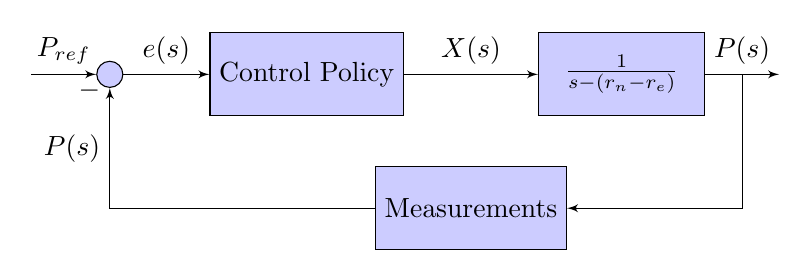
\begin{tikzpicture}[auto, node distance=2cm,>=latex']
	% We start by placing the blocks
	\node [input, name=input] {};
	\node [sum, right of=input] (sum) {};
	\node [block, right of=sum, node distance=2.5cm] (controller) {Control Policy};
	\node [block, right of=controller, node distance=4cm] (system) {$\frac{1}{s-(r_n-r_e)}$};
	% We draw an edge between the controller and system block to 
	% calculate the coordinate u. We need it to place the measurement block. 
	\draw [->] (controller) -- node[name=u] {$X(s)$} (system);
	\node [output, right of=system] (output) {};
	\node [block, below of=u] (measurements) {Measurements};
	
	% Once the nodes are placed, connecting them is easy. 
	\draw [draw,->] (input) -- node {$P_{ref}$} (sum);
	\draw [->] (sum) -- node {$e(s)$} (controller);
	\draw [->] (system) -- node [name=y] {$P(s)$}(output);
	\draw [->] (y) |- (measurements);
	\draw [->] (measurements) -| node[pos=0.99] {$-$} node [near end] {$P(s)$} (sum);
	\end{tikzpicture}
	\caption{Classical engineering feedback control block diagram implemented for the modelled population system. Measurements in this hypothetical control system would come from government collected data on population which is prone to lag - this may require estimates to be used instead of true figures for the scheme to work.}
\end{figure}

The lower saturation limit comes from the fact that our immigration policy has no negative actuation - put simply, we cannot change the number of immigrants per year such that the rate is negative. This constraint is expressed mathematically in equation 13:
\begin{equation}
X(t) \geq 0
\end{equation}

The upper saturation limit is one which is imposed from our discussion on sustainable growth rates, in Section 2.2. The recommendation was that population growth should not exceed $1.7\%$. Mathematically, this is described as:
\begin{equation}
	\frac{dP(t)}{dt} < 0.017 \cdot P(t)
\end{equation}

In terms of the birth, death, and immigration rates, we can express the saturation constraint in (13) as follows:
\begin{equation}
X(t) \leq \big(0.017 - (r_n - r_e)\big) \cdot P(t)
\end{equation}

This saturation limit is dependent on the population size itself, however, if we note that under a controlled system population will be bounded by the initial population, $P(t)|_{t=0}$, and the desired set point, $P_{ref}$, we can reasonably estimate this limit by assuming a fixed population around the midpoint between $P(t)|_{t=0}$ and $P_{ref}$. There are two control cases that have been considered for this analysis. The first instance is when the desired population level is greater than the current population level. For this case it was assumed that the current population level was at 25 million, and the desired population level was at 30 million. The increase from 25 million to 30 million can be seen in Figure 8, and the immigration policy that achieved this can be seen in Figure 9. The other case that is considered is when the desired population level is below the current population level. In this case, it was assumed again that the current population level was 25 million, and the desired level was 20 million. The decrease from 25 million to 20 million can be seen in Figure 10, and the immigration policy that achieved this can be seen in Figure 11.

\begin{figure}[h]
	\begin{minipage}[t]{0.45\textwidth}
		\centering
		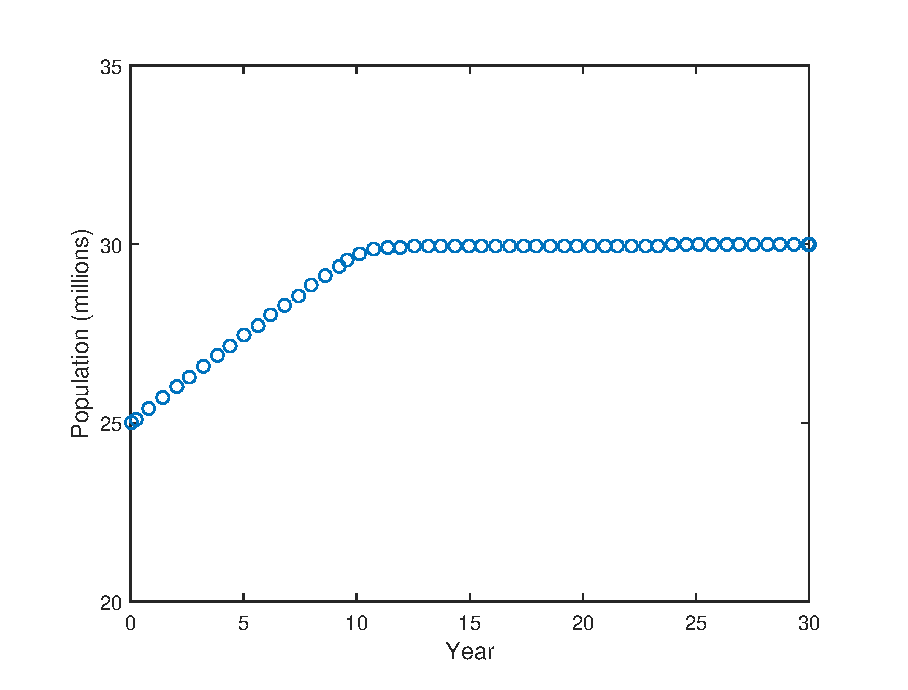
\includegraphics[scale=0.5]{population_control}
		\caption{The Australian population starts at 25 million and is increased to 30 million. Changes are made using immigration as a policy lever, under the assumption that natural rates of growth  and emigration remain constant.}
	\end{minipage}
	\hspace{1cm}
	\begin{minipage}[t]{0.45\textwidth}
		\centering
		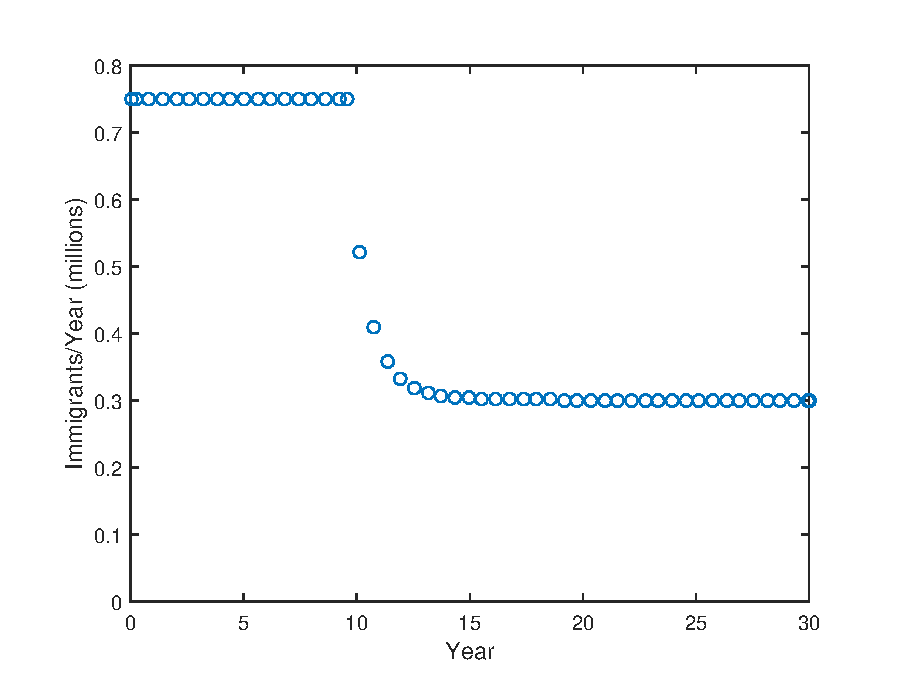
\includegraphics[scale=0.5]{immigration_policy}
		\caption{Immigration policy used to increase the Australian population from 25 million to 30 million.}
	\end{minipage}
\end{figure}

\begin{figure}[h]
	\begin{minipage}[t]{0.45\textwidth}
		\centering
		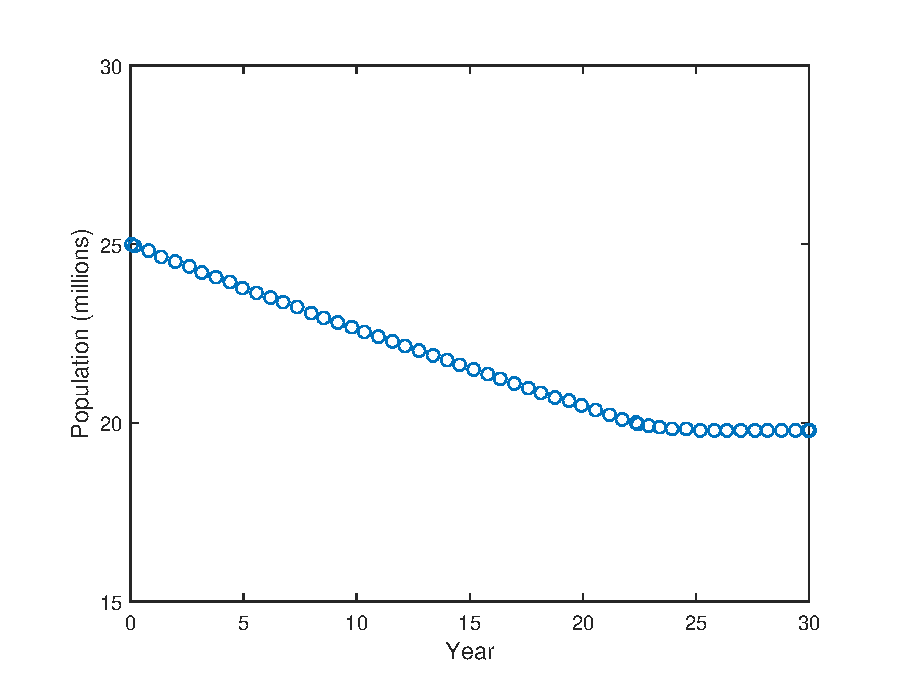
\includegraphics[scale=0.5]{population_control_2}
		\caption{The Australian population starts at 25 million and is decreased to 20 million. Changes are made using immigration as a policy lever, under the assumption that natural rates of growth  and emigration remain constant.}
	\end{minipage}
	\hspace{1cm}
	\begin{minipage}[t]{0.45\textwidth}
		\centering
		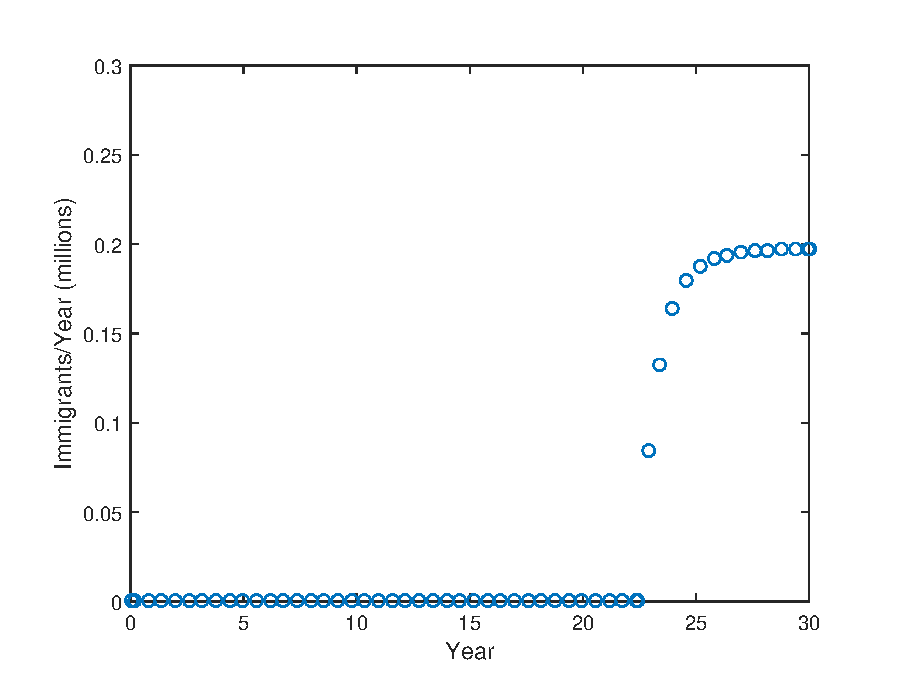
\includegraphics[scale=0.5]{immigration_policy_2}
		\caption{Immigration policy used to decrease the Australian population from 25 million to 20 million.}
	\end{minipage}
\end{figure}

\clearpage

\subsection{Analysis of Results}
In both cases presented above there exist demonstrated immigration policies which allow the government to achieve the desired population level. To raise the population level, the controller fully saturates to its upper limit of 750000 immigrants per year. Once the desired level is achieved, the immigration policy drops to around 300000 immigrants per year. Under the decreasing population scenario, we see a policy which is a little more extreme. Initially, the immigration policy is reduced to it's lower saturation limit of zero - this essentially stops permanent (or long term) immigration to Australia. The policy is held for approximately 20 years, until the desired population level is achieved and then immigration increases to allow approximately 200000 immigrants into Australia per year. It must be emphasised that the analysis presented in this section is not intended to be an immigration policy recommendation, rather it provides some insight into what options are available and how these options perform. Indeed, the immigration policies presented here are very aggressive. The simulated transition from a high level of immigration to a low level of immigration (or vice versa) occurs very rapidly. In reality, any such immigration control policy would see much softer transitions distributed over a greater number of years. Furthermore, in the population reduction scenario, despite the fact that there are some countries, like Japan (REFERENCE), that carry very restrictive immigration policies, it would be considered very aggressive to completely stop all immigration for an extended duration of time.\\

Perhaps the most important observation that can be gleaned from the modelling is the difference in time duration required to achieve the desired population level under the two different scenarios. Notably, the scenario which sees an increase in the population occurs more rapidly than the scenario in which the population level is decreased. This should serve as a warning that a conservative approach should be adopted when implementing policy to increase the population - any mistakes take a longer time to unwind and may require implementation of extreme policy measures.


%------------------------------------------------------------
\section{Impact on Australia's Higher Education Sector}
There are currently 43 Universities in Australia \cite{SMH1:2017}, which contribute a \$140 billion spend in the economy, and generate over \$12 billion in export revenue from international students \cite{GO8:2017}. Australia's international education strategy predicts there will be a 45\% increase in onshore international student numbers by 2025 representing a further \$8.6 billion in revenue. Domestic enrolments have been increasing as well. The Labour government's demand driven funding system uncapped the number of Commonwealth Government Supported positions, which significantly increased participation among middle and upper class Australian residents \cite{Grattan:2013}. This has led to increased pressure on the HECS-HELP loan scheme, with claims that the current level of spending is unsustainable. The current Liberal government have recently taken action on these claims by lowering the threshold for repayment to recoup outstanding loans amounts earlier. Additionally they have re-introducing caps to the number of funded positions for domestic students \cite{AUSGOV:2018}.\\

At the same time Universities were receiving more funding for additional students, the government was reducing funding for research. This has led to the practice of Universities cross-subsidising research with funding provided for teaching - this is especially true for the Group of Eight \cite{GO8:2017}. Tighter margins has resulted in the need for Universities to implement greater cost saving measures \cite{Spence:2018}. More drastic forms of this can be seen in merger proposals like that between University of South Australia, and my own beloved University of Adelaide \cite{Hatcher:2018}. As it stands with the current funding environment, most Universities are financially sustainable provided they manage costs and plan for the future. But what happens if the government willingly changes the population level? There are two scenarios we need to consider here. The first is if the government decides to lower the population below our current level of 25 million, and the second is if the government decides to raise the population above the current 25 million level. Of course there is a third scenario in which the current population level is maintained, but we will assume that current conditions will persist for no change.

\subsection{Decreasing the Population Below 25 million}
Decreasing the population, under the proposed population policy in Section 2.3, would see permanent and long term immigration lowered for an extended period of time, based on the modelling. On the surface the reduction in immigration may appear like it would have a materially negative impact on the Higher Education sector, however, there is only a small subset of the international student cohort who are studying in Australia purely for permanent residency \cite{Gordon:2018}. The major impact on the sector would come from decreasing domestic enrolments. The current number of Higher Education providers in this scenario is not sustainable. It must be noted that the fall in domestic enrolments would happen slowly, and Universities would have time to adjust their strategies. These adjustments would most likely range from merger activities, to increased focus on international markets, or even a reduction in size and specialisation in certain disciplines. 

\subsection{Increasing the Population Above 25 million}
Increasing the population, under the population policy outlined in Section 2.3, would see permanent and long term immigration increased for a period of time and then return to normalised levels. As previously mentioned this would only result in a small change on the international cohort coming to Australia for study. The main change would be in the number of domestic students. If the current funding cap was maintained in perpetuity, this would result in an increasingly competitive market for student positions at tertiary education institutions. This results in an unsustainable situation due to increased levels of inequality. The most likely losers in this perpetual funding cap scenario would be prospective students with lower socio-economic backgrounds, who don't have the same advantages as those from middle and upper classes. Of course, if the funding cap were to be lifted then this would not be a problem. The main problem in an uncapped scenario would be ensuring that HECS-HELP loan scheme is managed sustainably. The sustainable management of the loan scheme is a matter of perspective - there will be proponents for the increased HECS-HELP loan scheme to support all those who desired a University education, and detractors as well. There are multiple sources which society could raise additional funding to support the increased loan scheme: health care, military, or aged pension spending cuts could be made. Or perhaps corporate taxes could be increased. Or individual taxes. At its core the decision to fund an increased HECS-HELP loan scheme (or not) is argument around what society values, and as such is beyond the scope of this paper.

%------------------------------------------------------------
\section{Conclusion}
Historical estimates of carrying capacities for Australia range between 20 to 50 million, however, due to the limitations of the metric the Australian government has been reluctant to officially estimate this figure. Without carrying capacity estimates, the government has been unable, or unwilling, to propose desirable population levels, or the growth rate by which to achieve them. Population levels which creep too high run the risk of becoming unsustainable and damaging Australia's ecosystem. Conversely, population levels that are not managed properly can lead to age structure imbalance, causing economic stresses on younger generations. This provides strong motivation to establish a desired population level, and determine the population growth policy to sustainably achieve them. This paper proposed desired population levels could be estimated using carrying capacity estimates, and that sustainable growth could be controlled using immigration rates for permanent immigrants. Using  immigration rates for permanent immigrants to control population is desirable as it has low impact on current freedoms enjoyed by Australian residents, and will not impact the market for short term immigration which is used to export Higher Education in Australia. Mathematical modelling undertaken demonstrated that control was possible using only immigration rates, assuming that our current birth, death, and emigration rates do not substantially change over the long term. Modelling also revealed that it is more difficult to reduce the population level than it is to increase it - decreases take a longer duration of time and require more extreme policies. This type of population control would need to be periodically reassessed to incorporate new carrying capacity estimates, and ensure that there are no material changes to underlying assumptions.\\

The implications for the Australian Higher Education sector are principally concentrated around domestic enrolments, with evidence provided that only small changes in demand would be seen from international student cohorts. This is because only a subset of these students are seeking permanent residence.Two scenarios were explored:
\begin{itemize}
	\item if the population decreases then the Australian Higher Education sector, at its current size, will no longer be sustainable and will be forced to contract. This will happen over an extended duration, however, giving Universities time to consider future strategies;
	\item if the population increases, then this will cause increased competition for capped University places, most likely resulting in increased inequality as middle and upper classes crowd out students from lower socio-economic backgrounds.
\end{itemize}

\newpage

\section{Appendix A}

\begin{figure}[h]
	\centering
	\includegraphics[scale=0.8]{population_model_1}
	\caption{Simulink model use to create data for the Malthusian population decacy shown in Figure 6.}
\end{figure}

\vspace{2cm}

\begin{figure}[h]
	\centering
	\includegraphics[scale=0.8]{population_model_2}
	\caption{Simulink model use to create data for the immigration policy controls, and the population responses shown in Figures 8, 9, 10, and 11}
\end{figure}

\newpage
%------------------------------------------------------------

%\section{References}
\nocite{*} % Insert publications even if they are not cited
\let\Section\section 
\def\section*#1{\Section{#1}}
\bibliographystyle{unsrt}
\bibliography{ref_list}\vspace{0.75in}

%------------------------------------------------------------





\end{document}